\subsection{Bivariate clustering: copy number calling in qPCR data}
%\subsection{Two dimensional clustering enables accurate copy number calling in qPCR data} 


%% Figure 1
\begin{figure}[h!]
  \centering
  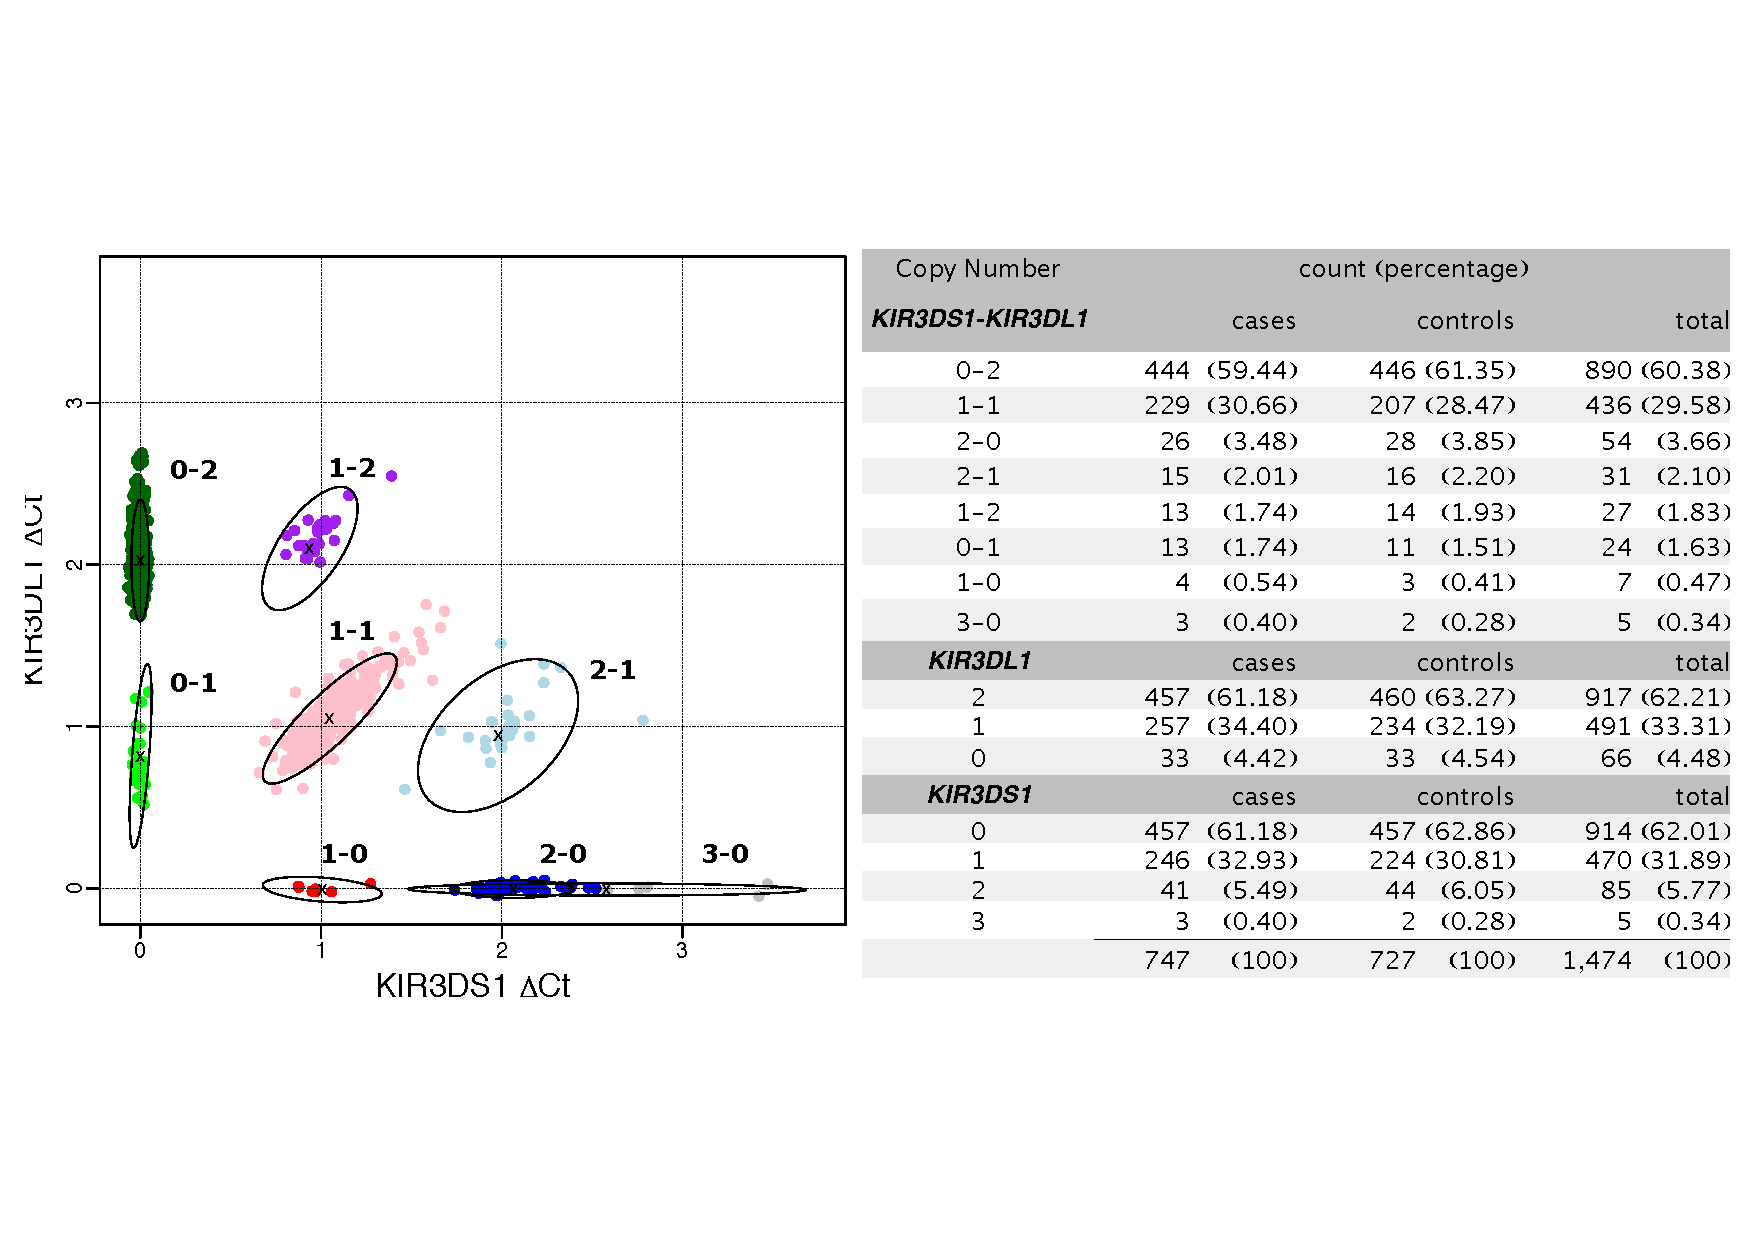
\includegraphics[scale=.5]{KIR/figures/Figure-1.pdf}
  \caption{ \label{Figure-1}
  \textbf{Copy number calling of \emph{KIR3DL1/3DS1} from qPCR $\Delta$Ct.}
  On the left, the median normalised $\Delta$Ct values for \emph{KIR3DS1} and
  \emph{KIR3DL1} are shown with the results of clustering into the eight
  copy number groups coloured according to the group with the
  highest posterior probability.  The three most common copy number groups are the
  ones with a total copy number of two: \emph{KIR3DL1} 0-2 (dark green),
  \emph{KIR3DL1/3DS1} 1-1 (pink) and \emph{KIR3DS1} 2-0 (dark
  blue).  The ellipses delimit the $95^{th}$ percentile.  On the right, the
  counts of the most probable copy number state are shown for cases and
  controls.}
\end{figure} 

Samples which yielded one or less Ct reading for Fam-KIR3DL1 or
Cy5-KIR3DS1, but all four Ct readings for the reference DFO-STAT6,
were assumed to contain zero copies of \emph{KIR3DL1} or
\emph{KIR3DS1}.  For the remainder of the samples, we called copy number groups
by fitting a mixture of bivariate Gaussian distributions to the two
dimensional normalised $\Delta$Ct values, allowing for eight
\emph{KIR3DS1/3DL1} copy number groups: three common groups of two copy
numbers (0-2, 1-1, 2-0) and five
rarer groups of lower or higher copy numbers
(Figure~\ref{Figure-1}).  The mixture was fitted using
an EM algorithm \citep{Young:2009ty} with initial parameters
calculated from the clusters returned by k-means with centers set to
the eight expected locations of the copy number groups.
After fitting the mixture model each sample was assigned a posterior
probability of belonging to each of the eight copy number groups which
allows for uncertainty in copy number calling.  These posterior
probabilities were taken into account in downstream statistical
analysis via multiple imputation.

Raw median $\Delta$Ct distributions varied across plates which prevented simple visual copy number assignment (Figure~\ref{Figure-S1}).
After normalisation, samples repeated across different plates showed good reproducibility (Figure~\ref{Figure-S3}) and two dimensional clustering enabled 1474 samples to be confidently assigned to a single copy number group, including all samples with known copy number which were assigned to the correct cluster.

%Firstly, we obtained posterior probabilities by fitting bivariate Gaussian distributions to our normalised combined KIR3DS1 and KIR3DL1 $\Delta$Ct values.
Jointly clustering on \emph{KIR3DL1} and \emph{KIR3DS1}, has the advantage of exploiting the correlation between the $\Delta$Ct values. 
For example, this can be seen in plate 10, where noisy cases (Figure~\ref{Figure-S1}.f) are difficult to assign as one or two copies based solely on their \emph{KIR3DL1} $\Delta$Ct, but are much more clearly distinguishable when we also consider their \emph{KIR3DS1} $\Delta$Ct value (Figure~\ref{Figure-S2}).
%For example, this can be seen in plate 10, where noisy cases (Figure~\ref{Figure-S1}) are hard to assign as one or two copies based solely on their \emph{KIR3DL1} $\Delta$Ct, but are much more clearly distinguishable when we also consider their \emph{KIR3DS1} $\Delta$Ct value (Figure~\ref{Figure-S2}).

%We allowed for the limited uncertainty of copy number calling by means of multiple imputation.


\begin{figure}[h]
    \centering
        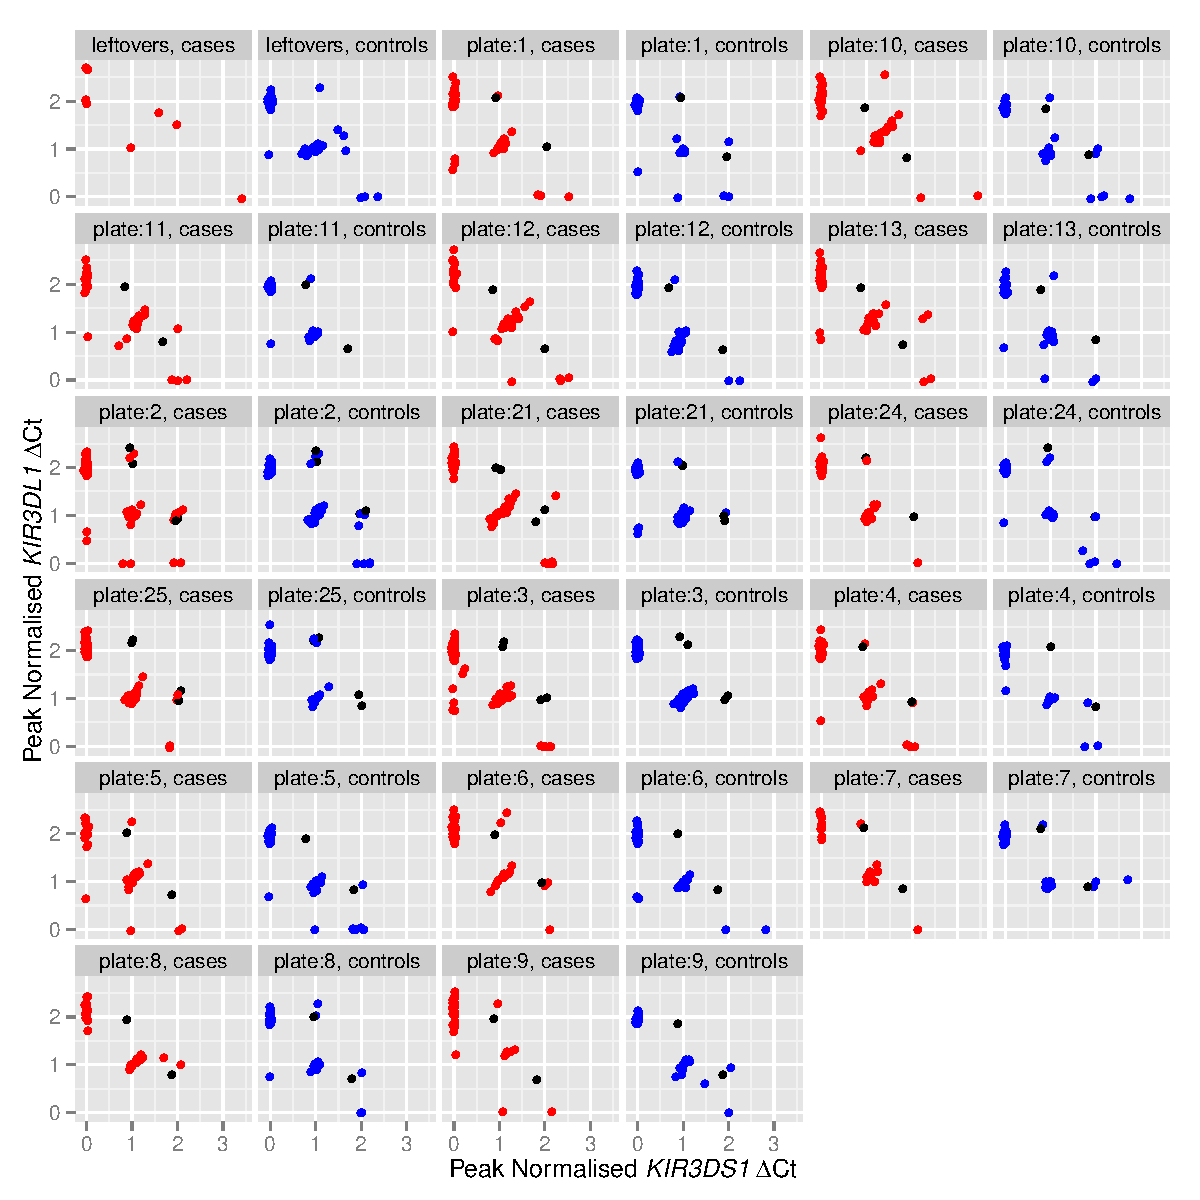
\includegraphics[scale=.9] {KIR/figures/Figure-S2.pdf}
    \caption{
        \label{Figure-S2}
        \textbf{Post-QC cases (red) and controls (blue) are plotted separately for each qPCR plate.}
        The samples with known \emph{KIR3DL1/3DS1} copy number are plotted in black.
        We can see that there is a larger spread in cases than in controls which is especially clear in the 1-1 copy number group.
        Also, it is apparent that the $\Delta$Ct of \emph{KIR3DL1} and \emph{KIR3DS1} are correlated in the 1-1, 2-1 and 1-2 groups.
        We exploited this correlation in the copy number calling by doing bivariate clustering.
    }
\end{figure}



\begin{figure}[h]
    \centering
    \begin{subfigure}[b]{.4\textwidth}
        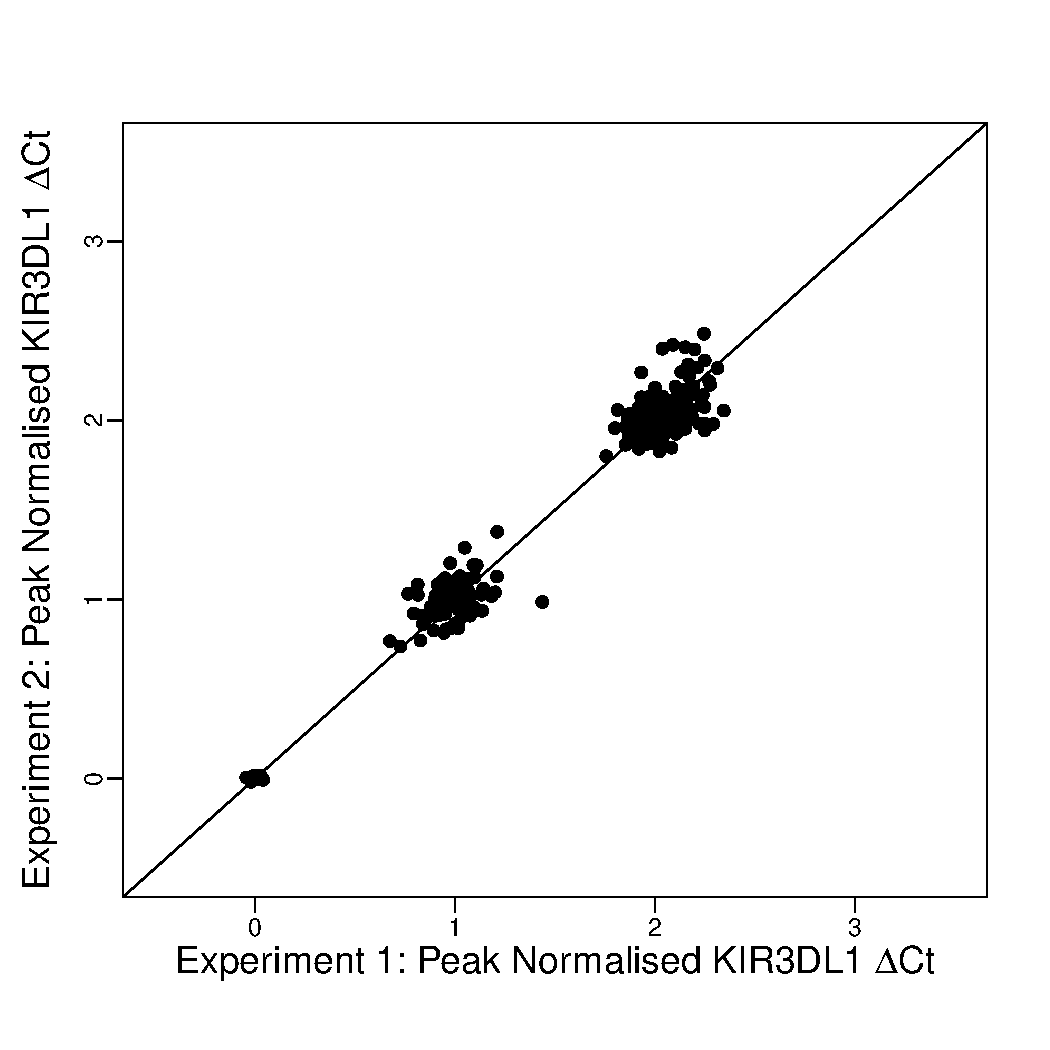
\includegraphics[scale=.4] {KIR/figures/DL1-repeatability.pdf}
        \caption{Repeatability of \emph{KIR3DL1} $\Delta$Ct post normalisation and QC ($r^{2}=0.961$).}
    \end{subfigure}
    ~
    \begin{subfigure}[b]{.4\textwidth}
        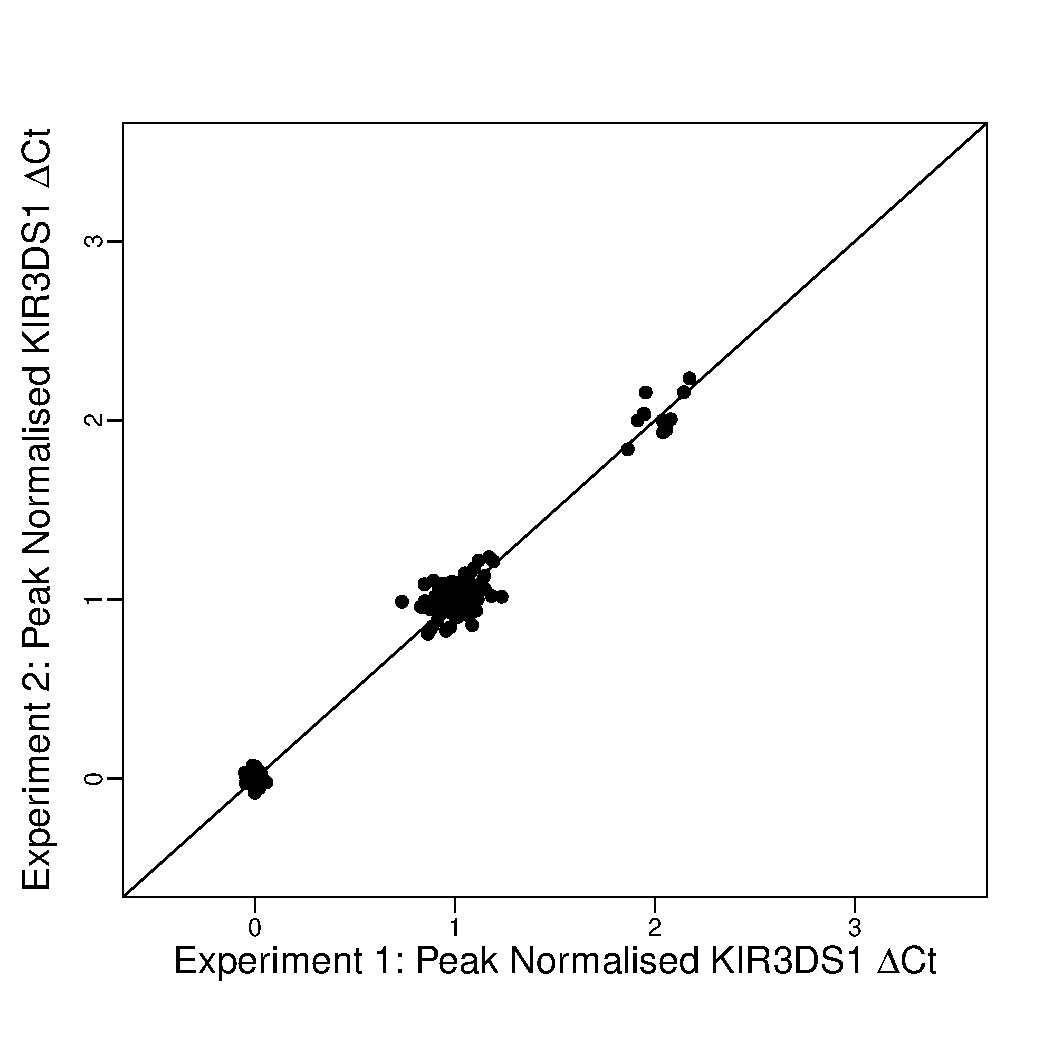
\includegraphics[scale=.4] {KIR/figures/DS1-repeatability.pdf}
        \caption{Repeatability of \emph{KIR3DS1} $\Delta$Ct post normalisation and QC ($r^{2}=0.99)$.}
        \label{}
    \end{subfigure}
    \caption{
        \label{Figure-S3}
        In order to assess the reliability of the qPCR assay 310 samples were re-analysed.
        We found very high reproducibility of the $\Delta$Ct values ($r^{2} > 0.96)$ confirming the reliability of our qPCR assay.
        %Samples on four plates were repeated to assess 
        %The points are coloured by genotype group as defined in Figure~\ref{figure:fuzzy-genotyping}.
        %302 samples
    }
\end{figure} 




\subsection{KNN classification: copy number imputation into the SNP data}
%\subsection{Copy number imputation into extended samples by integration of SNP array data and qPCR data} 

%% Figure 2
\begin{figure}[h!]
  \centering
  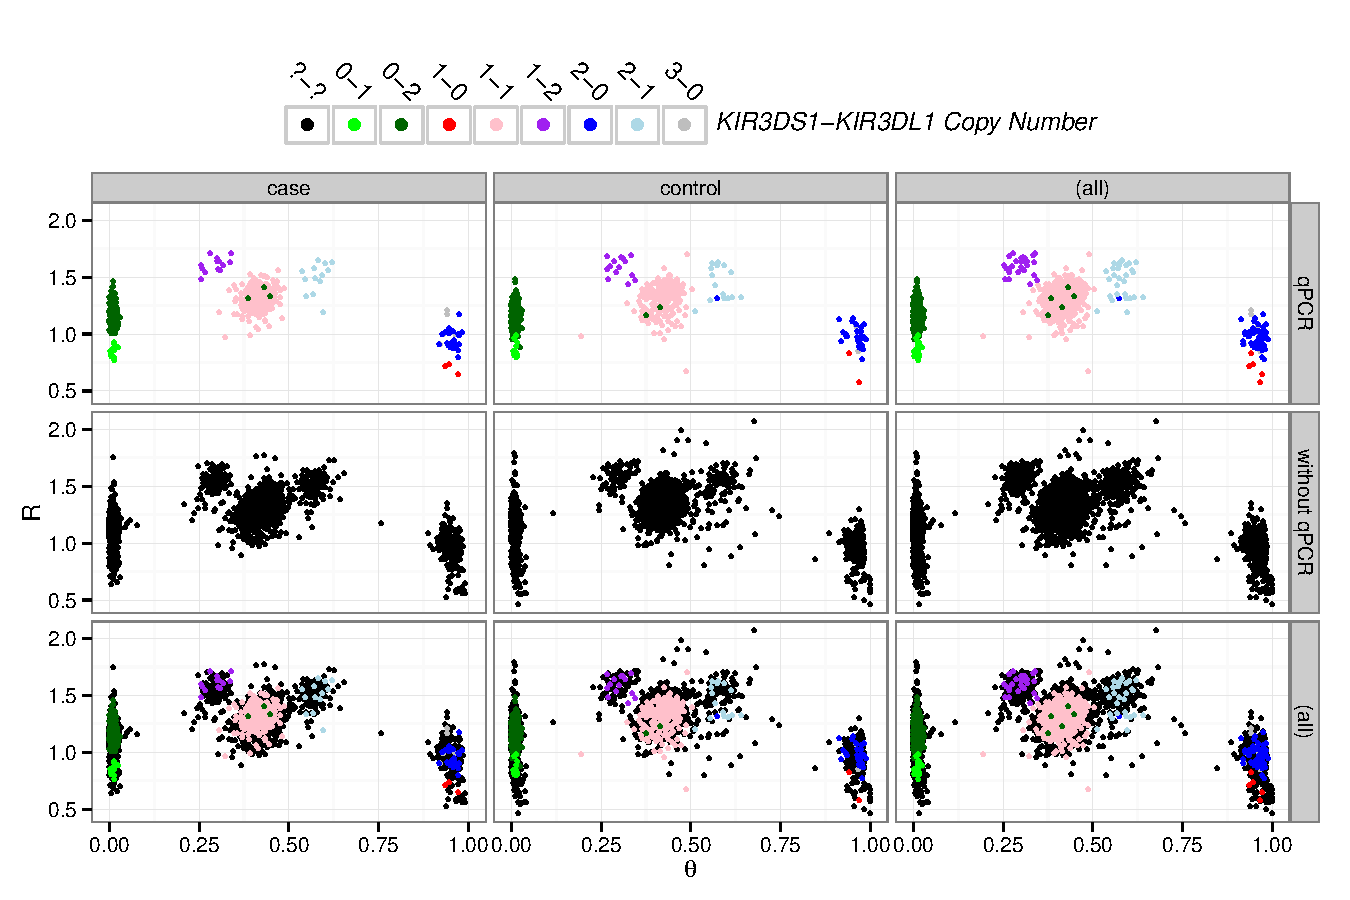
\includegraphics[scale=.5]{KIR/figures/Figure-2.pdf}
  \caption{ \label{Figure-2}
  \textbf{Overlay of ImmunoChip and qPCR samples for $R$ and $\theta$ at SNP rs592645.}
  Samples are coloured by the most likely \emph{KIR3DS1-KIR3DL1} copy number
  group according to the qPCR analysis (see Figure~\ref{Figure-1}).  The
  first and second row split the samples on the availability of qPCR data, and
  the third row is the overlay of the samples from the first and second row.
  The first and second column split the samples by case-control status and the
  third column is the overlay of the samples from the first and second column.}
\end{figure}

We extended our sample size by using the subset of samples common between the qPCR and SNP datasets, 747 cases and 727 controls, to train a k-nearest neighbour (knn) classifier to predict \emph{KIR3DL1/3DS1} copy number using the $R$ and $\theta$ signals from ImmunoChip SNPs.

Each of 30 SNPs lying within the \emph{KIR3DL1/3DS1} region were assessed for association with either \emph{KIR3LD1} or \emph{KIR3DS1} copy number in individual linear regression of copy number against $R$ and $\theta$ (Table~\ref{Table-S4}).
%Nineteen SNPs were significantly associated (Table~\ref{Table-S4}), with rs592645 the most strongly predictive (Figure~\ref{Figure-2}).
SNP signals, $R$ and $\theta$, showed strong association with individual copy numbers of \emph{KIR3DL1/3SD1} for nineteen of 30 SNPs in the \emph{KIR3DL1} region (Table~\ref{Table-S4}).
The strongest example is shown in Figure~\ref{Figure-2}, in which seven clusters for SNP rs592645 can be discerned that correspond closely with qPCR derived \emph{KIR3DL1/3SD1} copy numbers.
This figure also illustrates a number of important points about using SNP signals for imputation.
First, $\theta$ corresponds to the ratio of copies of \emph{KIR3DL1} to \emph{KIR3DS1}, while $R$ corresponds to the total copy number.
Second, some clusters overlap; without the qPCR data, the number of clusters and their boundaries would be difficult to define, particularly along the $R$ axis.
Finally, the clusters are in slightly different positions in cases and controls, reflecting the known sensitivity of genotyping chips to subtle differences in DNA preparation and storage conditions.
This has two implications: probabilistic clustering of the SNP data alone is likely to be poor in the combined sample, while unsupervised clustering of cases and controls separately when clusters are not clearly separated risks increasing type 1 error rates \citep{Plagnol:2007dw}.
Instead, we used the qPCR copy numbers as training data to perform supervised clustering of the SNP signals.

We first explored the validity of our imputation approach by means of leave-one-out cross-validation (LOOCV) in the samples with qPCR data.
We examined using all nineteen predictive SNPs, or various subsets, and found optimal knn imputation was achieved with the single most predictive SNP, rs592645 with $k=8$, which minimised the mean LOOCV error rate to \SI{2.0}{\percent} across ten multiply imputed qPCR datasets (Figure~\ref{Figure-3}).  

We also explored the effect of varying the size of the training data set by setting KIR gene copy numbers to missing for a randomly chosen subset of samples and imputing them in the remaining samples.
We suggest that only 295 samples are required to achieve LOOCV error rates $<5\%$ and 590 for error rates $<2.5\%$ (Figure~\ref{Figure-4}).


\rowcolors{2}{white}{white} 
\begin{table}[h]
\begin{center}
\footnotesize
\begin{tabular}{rlrllrr}
  \hline
Name                    & Position & SNP   & QC          & p-value $\theta$  & p-value R \\
  \hline
seq-rs597598            & 60007252 & [A/G] & ok          & 3.19E-03 & 7.81E-01 \\
seq-rs598452            & 60007428 & [A/G] & ok          & 6.53E-01 & 2.62E-01 \\
\rowcolor{LightCyan}
seq-t1d-19-60007809-C-G & 60007809 & [G/C] & ok          & 3.64E-02 & 6.27E-06 \\
seq-rs55761930          & 60008141 & [T/C] & ok          & 6.33E-01 & 6.12E-01 \\
\rowcolor{LightCyan}
seq-rs10500318          & 60012591 & [A/G] & ok          & 7.59E-11 & 1.31E-13 \\
\rowcolor{LightCyan}
seq-rs592645            & 60012739 & [A/T] & ok          & 8.85E-01 & 3.38E-09 \\
seq-rs604077            & 60013208 & [A/G] & ok          & 4.82E-03 & 1.20E-01 \\
\rowcolor{LightCyan}
seq-rs604999            & 60013409 & [A/G] & ok          & 1.77E-15 & 9.99E-04 \\
\rowcolor{LightCyan}
seq-t1d-19-60014013-A-C & 60014013 & [T/G] & lowcallrate & 8.74E-01 & 3.15E-08 \\
\rowcolor{LightCyan}
rs3865507               & 60014188 & [T/G] & ok          & 8.62E-03 & 6.93E-17 \\
\rowcolor{LightCyan}
seq-rs3865510           & 60016051 & [A/C] & ok          & 2.23E-10 & 2.04E-10 \\
seq-rs648689            & 60016286 & [A/G] & ok          & 2.31E-01 & 1.03E-02 \\
\rowcolor{LightCyan}
seq-rs649216            & 60016447 & [T/C] & ok          & 2.85E-02 & 1.04E-13 \\
\rowcolor{LightCyan}
rs581623                & 60018551 & [A/G] & ok          & 3.76E-02 & 2.06E-13 \\
\rowcolor{LightCyan}
seq-rs4806568           & 60022568 & [A/G] & lowcallrate & 1.44E-20 & 2.93E-01 \\
seq-rs674268            & 60024002 & [T/C] & lowcallrate & 1.43E-02 & 2.90E-01 \\
rs12461010              & 60024413 & [A/G] & ok          & 4.72E-01 & 1.72E-01 \\
\rowcolor{LightCyan}
seq-rs2295805           & 60028513 & [T/C] & lowcallrate & 9.55E-08 & 8.40E-04 \\
seq-rs12976350          & 60030391 & [T/C] & lowcallrate & 1.70E-05 & 5.07E-01 \\
seq-t1d-19-60034052-C-T & 60034052 & [A/G] & hwe         & 3.27E-02 & 4.07E-01 \\
\rowcolor{LightCyan}
rs4806585               & 60038236 & [T/G] & hwe         & 2.20E-11 & 2.42E-02 \\
\rowcolor{LightCyan}
seq-rs62122181          & 60039178 & [T/C] & lowcallrate & 2.40E-13 & 2.26E-01 \\
rs10422740              & 60052298 & [T/C] & monomorph   & 7.78E-01 & 8.49E-02 \\
\rowcolor{LightCyan}
rs640345                & 60054671 & [A/G] & ok          & 3.61E-07 & 6.83E-02 \\
seq-t1d-19-60054973-T-C & 60054973 & [A/G] & ok          & 2.92E-01 & 2.28E-04 \\
\rowcolor{LightCyan}
seq-t1d-19-60056605-A-T & 60056605 & [A/T] & ok          & 3.99E-01 & 1.48E-16 \\
\rowcolor{LightCyan}
seq-t1d-19-60056721-C-T & 60056721 & [A/G] & ok          & 9.02E-01 & 2.04E-09 \\
\rowcolor{LightCyan}
seq-rs10407958          & 60063974 & [T/A] & ok          & 1.06E-02 & 5.45E-10 \\
\rowcolor{LightCyan}
seq-rs1654644           & 60065174 & [T/G] & ok          & 7.94E-14 & 5.21E-12 \\
\rowcolor{LightCyan}
rs3826878               & 60069023 & [A/G] & ok          & 2.63E-05 & 3.55E-06 \\
   \hline
\end{tabular}
%xtable(kir, display=c('d','s','d','s','s','E','E')) 
\end{center}
    \caption{
    \label{Table-S4}
        The 30 ImmunoChip SNPs which fall in the \emph{KIR3DL1} region according to build36/hg18, nineteen of which
        are significantly associated with \emph{KIR3DL1/3DS1} copy number (highlighted in blue).
        %\emph{KIR3DS1} is missing from build36/h18.
% GenCall Score:
%http://res.illumina.com/documents/products/technotes/technote_gencall_data_analysis_software.pdf
        %http://www.biomedcentral.com/1471-2105/12/68
    }
\end{table}


%% Figure 3
\begin{figure}[h!]
  \centering
  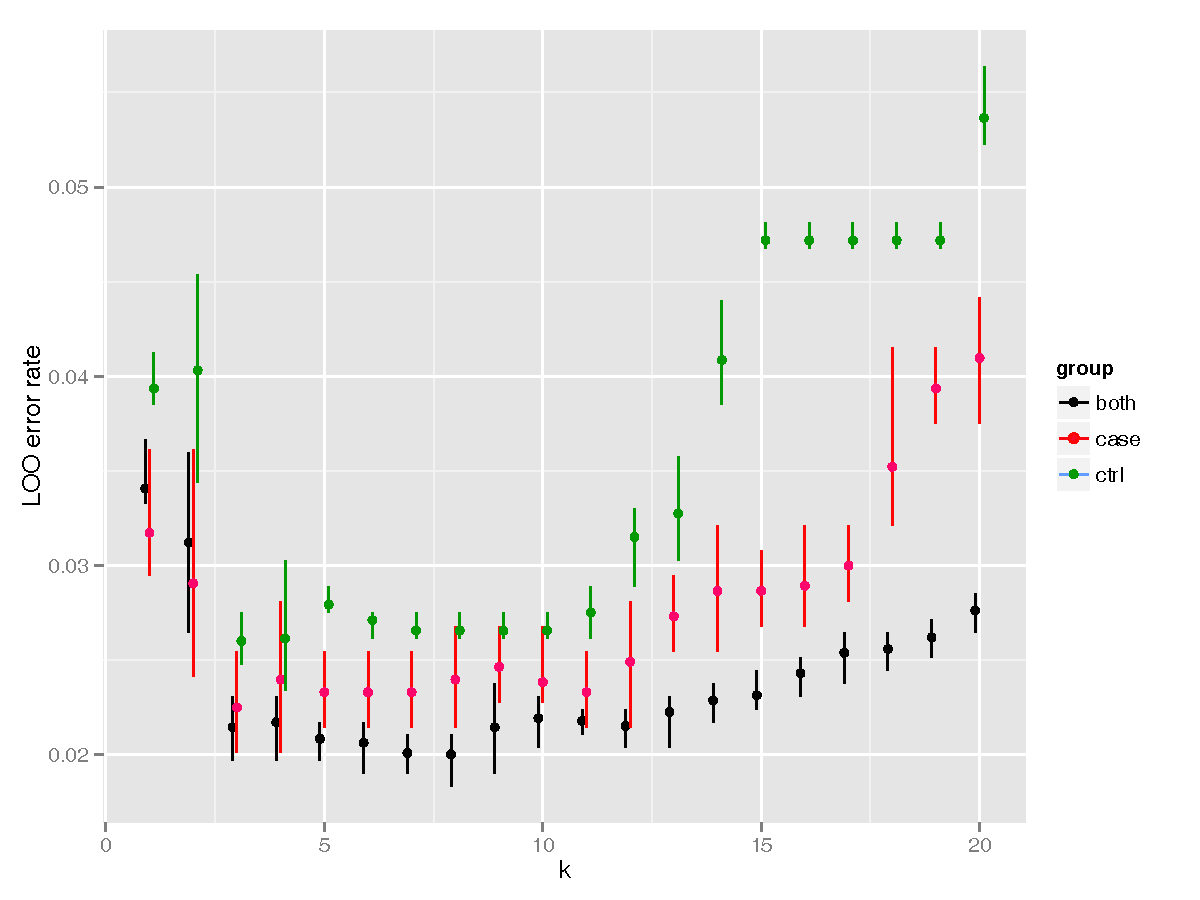
\includegraphics[scale=.5]{KIR/figures/Figure-3.pdf}
  \caption{ \label{Figure-3}
  \textbf{Leave-one-out crossvalidation error rate for k-nearest neighbour prediction.}
  Leave-one-out cross validation error rates
  obtained from k-nearest neighbours (knn) prediction
  of \emph{KIR3DL1/3DS1} copy numbers from the $R$ and $\theta$ signals of SNP rs592645.
  Each point shows the proportion of samples for which the knn predicted copy number did not 
  match the qPCR call, averaged over ten multiply imputed qPCR call datasets
  (using the posterior probabilities from Figure~\ref{Figure-1}). 
  Error bars show the minimum and maximum error rates over the ten multiply imputed datasets.
  Knn was run in parallel for cases only, controls only and on all samples together.
  The minimum error rate is achieved for $k=8$ when the prediction uses both cases and controls.}
\end{figure}

%% Figure 4
\begin{figure}[h!]
  \centering
  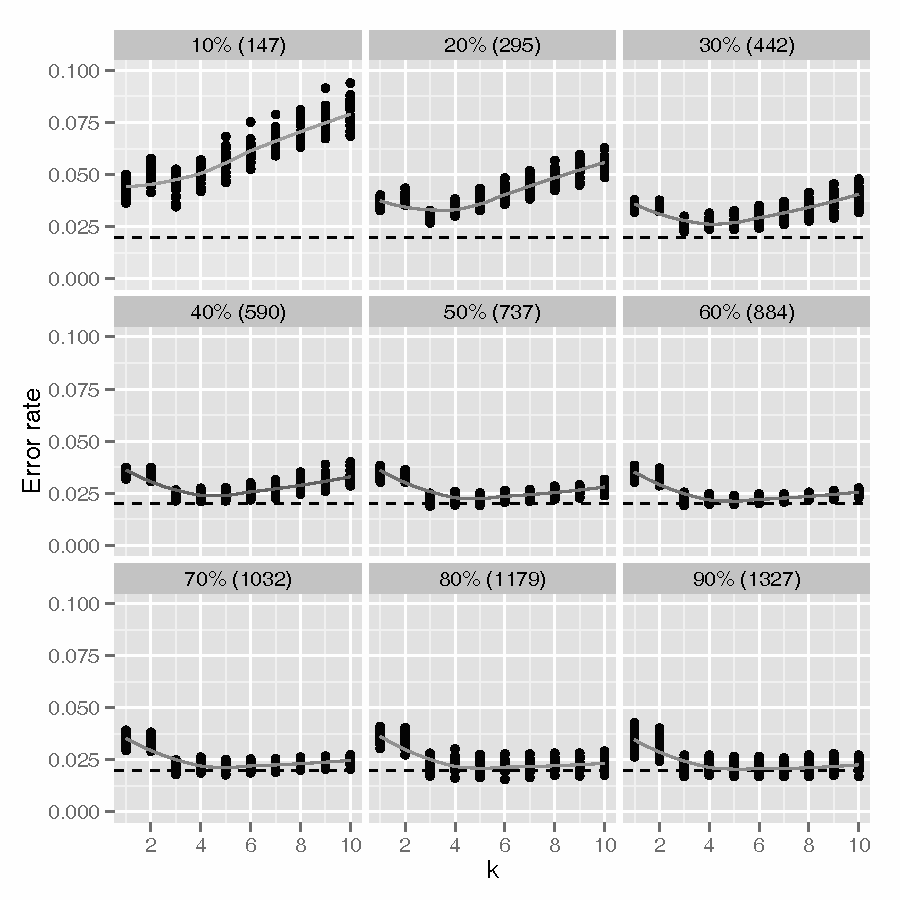
\includegraphics[scale=.5]{KIR/figures/Figure-4.pdf}
  \caption{ \label{Figure-4}
  \textbf{Error rate of k-nearest neighbour prediction from $R$ and $\theta$ of rs592645 in random subset of samples.}
  Each panel shows the LOOCV error rates of \emph{KIR3DL1/3DS1} copy number prediction
  from $R$ and $\theta$ of rs592645 in the remaining unlabeled samples
  when using a different size subset of the training data.
  The percentage of the complete training data set and the size of the subset is given in the title of each panel.
  Each point represents the LOOCV error rate averaged over ten multiply imputed qPCR call datasets
  (using the posterior probabilities from Figure~\ref{Figure-1}). 
  Smoothing lines show the average over 25 independent random subsets of training data.
  The black dashed line represent the observed error rate in the complete sample.
  As the size of the training dataset increases the error rate becomes less sensitive to the choice of the parameter k.
  Only 295 samples are required to achieve LOOCV error rates $<5\%$ and 590 for error rates $<2.5\%$.}
\end{figure}


